\clearpage
\subsection{Type (recap)} % (fold)
\label{sub:type_recap_}

This chapter is all about types, so its is important to have a good understanding of what a type is. A type is a specification for a class of data, describing how it is stored and interpreted.

\begin{figure}[h]
   \centering
   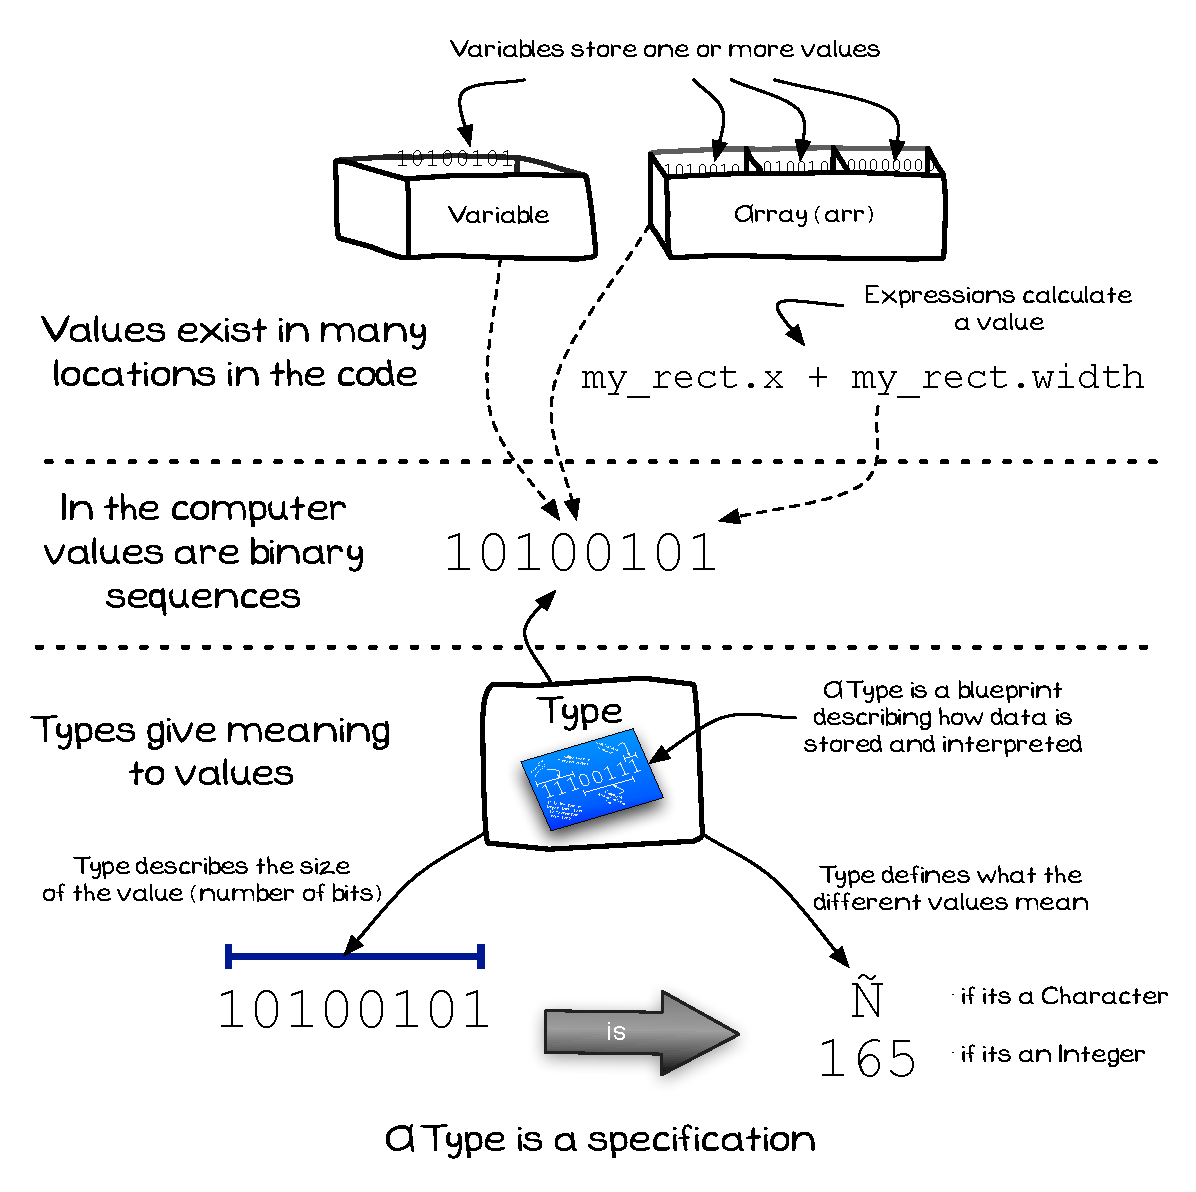
\includegraphics[width=\textwidth]{./topics/type-decl/diagrams/TypeRecap} 
   \caption{Type defines the size and interpretation if values in your code}
   \label{fig:type-recap}
\end{figure}

\mynote{
\begin{itemize}
  \item A Type is a kind of \texttt{artefact}, describing the format and interpretation of values.
  \item Types specify the following:
  \begin{itemize}
    \item The size (number of bits) needed to store values of this type.
    \item How the bits of the type are interpreted.
    \item The operations that can be performed on values of this type.
  \end{itemize}
  \item You can think of a Type as a blueprint, specifying data layout.
  \item The interpretation of a value depends on its Type, for example \texttt{10100101} is \~{N} if the value is a Character type, but the same value would be \texttt{165} if it is an Integer type.
  \item You can create your own types...
\end{itemize}
}

% subsection type_recap_ (end)